\section{Description of the achievements}

As of SageMath version 8.0, Sage is available for 64-bit versions of
Windows 7 and up. It can be downloaded through the SageMath website, and
up-to-date installation instructions are being developed at the SageMath
wiki\footnote{\url{https://wiki.sagemath.org/SageWindows}}.

The installer contains all software and documentation making up the standard
Sage distribution, all libraries needed for Cygwin support, a Bash shell,
numerous standard UNIX command-line utilities, and the MinTTY terminal
emulator, which is generally more user-friendly and better suited for
Cygwin/UNIX software than the standard Windows console.

It is distributed in the form of a single-file executable installer, with a
familiar install wizard interface. The download size of the installer comes in
at just under a gigabyte, but unpacks to more than 4.5 GB in version 8.0.

\begin{figure}[h!]
    \centering
    \begin{subfigure}[b]{0.45\textwidth}
        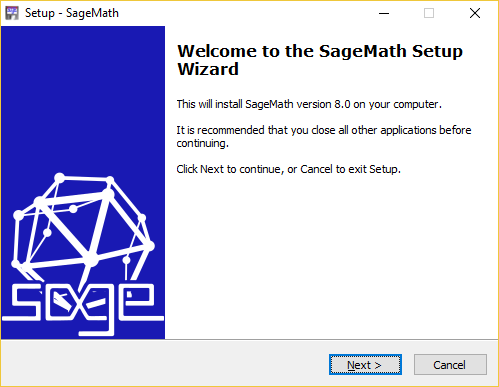
\includegraphics[width=\textwidth]{screenshots/installer1}
    \end{subfigure}
    ~
    \begin{subfigure}[b]{0.45\textwidth}
        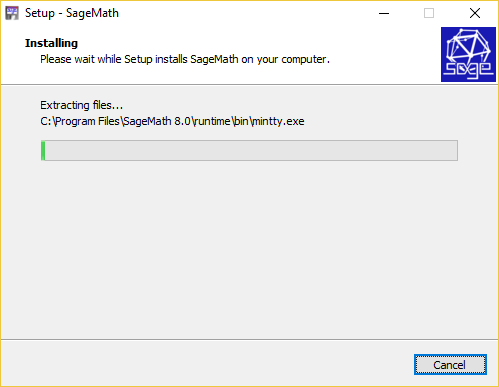
\includegraphics[width=\textwidth]{screenshots/installer2}
    \end{subfigure}
    \caption{SageMath for Windows installation}
    \label{fig:installation}
\end{figure}

Because of the large number of files comprising the complete SageMath
distribution, and the heavy compression of the installer, installation can take
a fair amount of time even on a recent system. On an Intel i7 laptop it takes
about ten minutes, but results will vary. Fortunately, after nearly a year of
field testing, this has not yet been a source of complaints.  In future updates
to the installer we may also be able to reduce the installation time/size by
making certain large components (e.g.~offline documentation) optional.

The installation also includes a graphical uninstaller that can be run in the
standard way via the control panel, as well as three desktop and/or start menu
shortcuts:

\begin{figure}[h!]
    \centering
    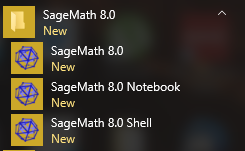
\includegraphics{screenshots/shortcuts}
    \caption{Shortcut icons for SageMath}
    \label{fig:shortcut-icons}
\end{figure}

\begin{enumerate}
\def\labelenumi{\arabic{enumi})}
\item
  The shortcut titled just ``SageMath 8.0'' launches the standard Sage
  command prompt in a text-based console. In general it integrates well
  enough with the Windows shell to launch files with the default viewer
  for those file types. For example, plots are saved to files and
  displayed automatically with the default image viewer registered on
  the computer.
\item
  ``SageMath Shell'' runs a Bash shell with the environment set up to
  run software in the Sage distribution. More advanced users, or users
  who wish to directly use other software included in the Sage
  distribution (e.g.~GAP, Singular) without going through the Sage
  interface.
\item
  ``SageMath Notebook'' starts a Jupyter Notebook server with Sage
  configured as the default kernel and, where possible, opens the
  Notebook interface in the user's browser.
\end{enumerate}

\begin{figure}[h!]
    \centering
    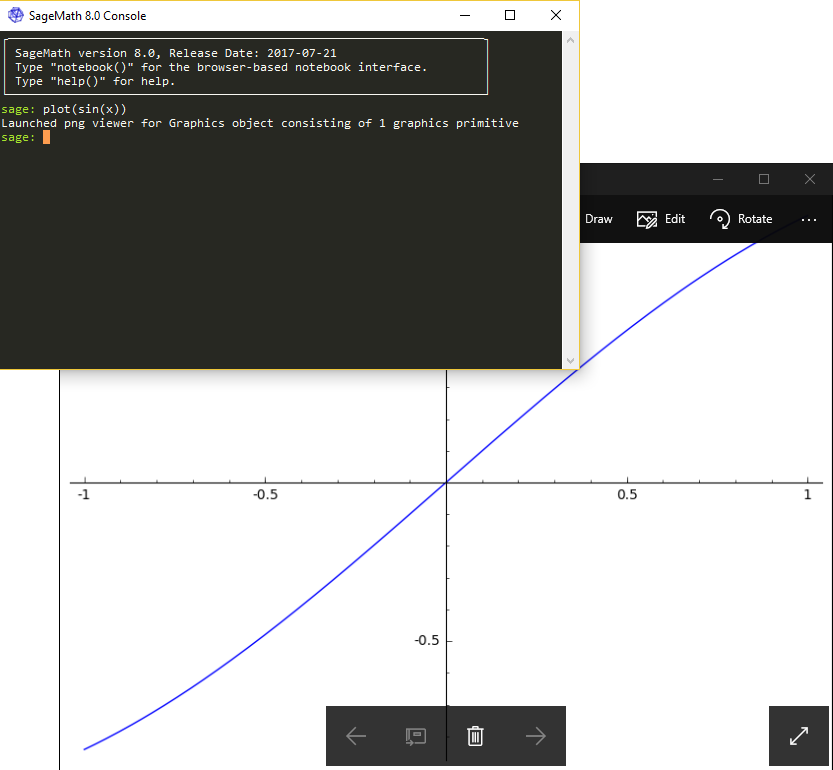
\includegraphics[width=\textwidth]{screenshots/console}
    \caption{SageMath text console with a plot in the default Windows image viewer}
    \label{fig:console}
\end{figure}

\section{Technical details}

The main challenge with porting Sage to Windows/Cygwin has relatively
little to do with the Sage library itself, which is written almost
entirely in Python/Cython and involves relatively few system interfaces.
Rather, most of the effort has gone into build and portability issues
with Sage's more than 150 dependencies.

The majority of issues have been build-related issues. Runtime issues
are less common, as many of Sage's dependencies are primarily
mathematical, numerical code. Another reason is that, although there are
some anomalous cases, Cygwin's emulation of POSIX interfaces is good
enough that most existing code just works as-is. However, because
applications built in Cygwin are native Windows applications and DLLs,
there are Windows-specific subtleties that come up when building some
non-trivial software. So most of the challenge has been getting all of
Sage's dependencies building cleanly on Cygwin, and then maintaining
that support (as the maintainers of most of these dependencies are not
themselves testing against Cygwin regularly).

In fact, maintenance was the most difficult aspect of the Cygwin port
(and this is one of the main reasons past efforts failed--without a
sustained effort it was not possible to keep up with the pace of Sage
development).

\subsection{Continuous integration}\label{continuous-integration}

A critical component that was missing for creating a sustainable Cygwin port of
Sage was continuous integration on Cygwin. The Sage developers maintain a
flotilla of so-called "patchbots", computers running a number of different OS
and hardware platforms that perform continuous integration testing of all
proposed software changes to Sage.  The patchbots are able to catch changes
that break Sage before they are merged into the main development branch.
Without a patchbot testing changes on Cygwin, there was no way to stop changes
from being merged that broke Cygwin. With some effort Erik Bray managed to get
a Windows VM with Cygwin running reliably on Université Paris-Sud's OpenStack
infrastructure, that could run a Cygwin patchbot for Sage. By continuing to
monitor this patchbot the SageMath community can now receive prior warning
if/when a change will break the Cygwin port. We expect this will impact only a
small number of changes--in particular those that update one of Sage's
dependencies.

In so doing we are, indirectly, providing continuous integration on
Cygwin for SageMaths's many dependencies--something most of those
projects do not have the resources to do on their own. So this should be
considered a service to the open source software community at large.


\subsection{Runtime bugs}\label{runtime-bugs}

Despite the relative lack of system-specific code in Sage, there were some
non-trivial bugs that occurred at run time (as opposed to during software
builds) that required considerable effort to debug resolve.

One particular source of bugs is subtle synchronization issues in multi-process
code, that arise primarily due to the large overhead of creating, destroying,
and signalling processes on Cygwin, as compared to most UNIXes.  Other problems
arise in areas of behavior that are not specified by the POSIX standard, and
assumptions are made that might hold on, say, Linux, but that do not hold on
Cygwin (but that are still POSIX-compliant!)  For example, a difference in
(undocumented, in both cases) memory management between Linux and Cygwin made
for a particularly challenging bug in PARI on
Cygwin\footnote{\url{https://trac.sagemath.org/ticket/22633}}.

Another interesting bug\footnote{\url{https://trac.sagemath.org/ticket/21388}}
came up in a test that invoked a stack overflow bug in Python, which only came
up on Cygwin due to the smaller default stack size of programs compiled for
Windows.  There are also occasional bugs due to small differences in numerical
results, due to the different implementation of the standard C math routines on
Cygwin, versus GNU libc.

It was also discovered in the process of porting to Cygwin that the Python
interpreter's support for thread-local data in multi-threaded programs was
fundamentally broken on Cygwin (due not to a problem in Cygwin, but to aspects
of the Python interpreter that were not POSIX-compliant).  Although the problem
was simple the fix was non-trivial, and led to Erik Bray co-authoring a Python
Enhancement Proposal
(PEP)\footnote{\url{https://www.python.org/dev/peps/pep-0539/}}--a technical
specification for communicating to the Python community some design or
implementation aspect of the Python language or its official interpreter
implementation, "CPython".

This leaves us with the lesson that porting software as complex as Sage and its
dependencies to Cygwin is not completely trivial, and that similar bugs might
still arise in the future, requiring future investment.  See
\ref{upstream-contributions} for a list of other open source projects that were
contributed to in the process of porting Sage to Cygwin/Windows.


\subsection{Alternatives}\label{alternatives}

There are a few possible routes to supporting Sage on Windows, of which
Cygwin is just one. For example, before restarting work on the Cygwin
port Erik Bray experimented with a solution that would run Sage on
Windows using Docker.
It was showcased at the first project review in
April 2017, and was advertised on SageMath's website as a temporary
alternate installation method for some time before the release of
SageMath 8.0.
This approach was relatively lightweight, and the prototype functional;
however it remained clumsy, and the final show stopper was that, on many
windows machine, the user had to first switch a flag in his BIOS
configuration, which made the installation suddenly much harder for
casual users.

Another approach, which was investigated in the early efforts to port Sage
to Windows, is to get Sage and all its dependencies building with
the standard Microsoft toolchain (MSVC, etc.). This would mean both
porting the code to work natively on Windows, using the MSVC runtime, as
well as developing build systems compatible with MSVC. There was a time
when, remarkably, many of Sage's dependencies did meet these
requirements. But since then the number of dependencies has grown too
much, and Sage itself become too dependent on the GNU toolchain, that
this would be an almost impossible undertaking with available resources.

A middle ground between MSVC and Cygwin would be to build Sage using the
MinGW toolchain, which is a port of GNU build tools (including binutils,
gcc, make, autoconf, etc.) as well as some other common UNIX tools like
the Bash shell to Windows. Unlike Cygwin, MinGW does not provide
emulation of POSIX or Linux system APIs. This would actually be the
preferred approach, and with enough time and resources it could probably
work. However, it would still require a significant amount of work to
port some of SageMath's more non-trivial dependencies, such as GAP and
Singular, to work on Windows without some POSIX emulation. Now that the
Cygwin port has been completed, a MinGW port seems more feasible.

Finally, a note on the Windows Subsystem for Linux (WSL), which debuted shortly
after the start of OpenDreamKit. The WSL is a new effort by Microsoft to allow
running executables built for Linux directly on Windows, with full support from
the Windows kernel for emulation of Linux system calls. Basically, it aims to
provide all the functionality of Cygwin, but with full support from the kernel,
and the ability to run Linux binaries directly without having to recompile
them. This is a very promising development. Thus, the question is asked if Sage
can run in this environment, and experiments suggest that it works, albeit
imperfectly (the WSL is still under active development by Microsoft and some of
its interfaces are less robust than others).

A detailed account of WSL was already given in deliverable D2.3
(September 2016). In short:
\begin{enumerate}
\def\labelenumi{\arabic{enumi})}
\item The WSL is currently only intended as a developer tool: there is no way
    to package Windows software for end users such that it uses the WSL
    transparently, and users must install Microsoft development tools in order
    to use WSL.

\item It is only available on recent updates of Windows 10--it will never be
    available on older Windows versions.
\end{enumerate}

So to reach the most users, and provide the most hassle-free user experience,
the WSL is not currently a solution.  However, it may still prove useful for
developers as a way to do Sage development on Windows. And in the future it may
become the easiest way to install UNIX-based software on Windows as well,
especially if Microsoft ever expands the scope of its supported use cases. It
may also lead to improvements in the implementation of Cygwin if Microsoft is
ever more forthcoming about some of the WSL's implementation details.


\section{Upstream contributions}\label{upstream-contributions}

As discussed previously, while relatively little code in the Sage library is
platform-dependent, a significant number of Sage's dependencies have had bugs
with building and running on Cygwin.  Thus, the effort of porting Sage to
Cygwin involved upstream improvements to numerous other open source projects
including but not limited to:

\begin{enumerate}
\item Cygwin itself (fixes to bugs in Cygwin that affected Sage)
\item Python (fixes to bugs with using Python on Cygwin)
\item PyCygwin\footnote{\url{https://github.com/embray/PyCygwin}} (a project we created for interfacing with Cygwin's internals from Python)
\item Cysignals
\item psutil (a popular multi-platform process monitoring library for Python, which required some effort to port to Cygwin)
\item OpenBlas (the default linear algebra library used by Sage)
\item ECL (Extensible Common Lisp, on top of which Maxima is developed)
\item ECM (used for elliptic curve factorization)
\item cddlib
\item fplll
\item GAP
\item libhomfly
\item Linbox
\item NumPy
\item PARI/GP
\item Singular
\end{enumerate}

As mentioned previously, Erik Bray also co-authored a Python Enhancement
Proposal (PEP) that was accepted and implemented in Python 3.7.  They also
contributed to improving the port of Python 3 to Cygwin, and in the process
were also given elevated privileges on the CPython project's main issue tracker
with the purpose of managing Cygwin-related issues on Python.


\section{Port for 32 bits architectures}\label{port-for-32-bits-architectures}

Until 2013 the only available version of Cygwin was for 32-bit
architectures. The original goal of the deliverable was to make
Cygwin-based installers both for 32- and 64-bit architectures. After
getting Sage working on 64-bit Cygwin, when it came time to test on
32-bit Cygwin we hit some significant snags.

The main problem is that 32-bit Windows applications have a user address
space limited to just 2 GB. This is in fact not enough to fit all of
SageMath into memory at once. With some care, such as reserving address
space for the most likely to be used (especially simultaneously)
libraries in Sage, we could work around this problem for the average user.
But the result may still not be 100\% stable.

It becomes a valid question whether this is worth the effort. There are
unfortunately few publicly available statistics on the current market
share of 64-bit versus 32-bit Windows versions among desktop users. Very
few new desktops and laptops sold anymore to the consumer market include
32-bit OSes, but it is still not too uncommon to find on some older,
lower-end laptops. In particular, some laptops sold not too long ago
with Windows 7 were 32-bit. According to Net Market Share\footnote{\url{https://www.netmarketshare.com/operating-system-market-share.aspx?qprid=10\&qpcustomd=0}},
as of writing Windows 7 still makes up nearly 50\% of all desktop
operating system installments. This still does not tell us about 32-bit
versus 64-bit. The popular (12.5 million concurrent users) Steam PC
gaming platform publishes the results of their usage statistics
survey\footnote{\url{http://store.steampowered.com/hwsurvey/}}, which as
of writing shows barely over 5\% of users with 32-bit versions of
Windows. However, computer gamers are not likely to be representative of
the overall market, being more likely to upgrade their software and
hardware.

Given the lack of demand for 32-bit versions of SageMath on Windows, the
continually shrinking market share of such systems, and the availability of
legacy installation methods for them, we have decided not to pursue this effort
further. Should a serious use case for such a port eventually arise, we may
have to reconsider our decision.

\section{Conclusion}\label{conclusion}

Focusing on Cygwin for porting Sage to Windows was definitely the right way to
go. It took roughly three months in the summer of 2016 to get the vast majority
of the initial work done, with sustained effort over the following two years in
order to keep up with changes to Sage and fix some of the more obscure bugs.
We estimate an overall expenditure of 14 person-months on this effort, tracked
across roughly 115 tickets on Sage's bug tracker as of
writing\footnote{\url{https://trac.sagemath.org/report/94}}.

Now, however, enough issues have been addressed that the Windows version has
remained fairly stable, even in the face of ongoing updates to Sage. Because
some effort is required in order to maintain the continuous integration of Sage
on Cygwin, build releases, and address new issues that arise, a sustained
effort of roughly 2 person-months annually is required, with likelihood that
that will continue to decrease as software stability improves.

Porting more of Sage's dependencies to build with MinGW and without Cygwin
might still be a worthwhile effort, as Cygwin adds some overhead and stability
issues in a few areas, but if we had started with that approach it would have
taken much longer to produce usable results.

In the near future, however, the priority needs to be improvements to
user experience of the Windows installer. In particular, a better
solution is needed for installing Sage's optional packages on Windows.
And an improved experience for using Sage in the Jupyter Notebook, such
that the Notebook server can run in the background as a Windows Service,
would be desirable. This feature would not be specific to Sage either, and
could benefit all users of the Jupyter Notebook on Windows.
